\documentclass[12pt, twoside]{article}
\usepackage[francais]{babel}
\usepackage[T1]{fontenc}
\usepackage[latin1]{inputenc}
\usepackage[left=4mm, right=4mm, top=4mm, bottom=4mm]{geometry}
\usepackage{float}
\usepackage{graphicx}
\usepackage{array}
\usepackage{multirow}
\usepackage{amsmath,amssymb,mathrsfs} 
\usepackage{soul}
\usepackage{textcomp}
\usepackage{eurosym}
\usepackage{lscape}
 \usepackage{variations}
\usepackage{tabvar}
 
\pagestyle{empty}


\begin{document} 

\begin{center}
\Large{\ul{\textbf{Fonctions affines}}}
\end{center}


\section{D�finitions et exemples}

\ul{D�finition:} Une \textbf{fonction affine} est une fonction qui � un nombre
$x$ associe le nombre $ax+b$ avec $a$ et $b$ deux nombres donn�s.

On note: \ldots \ldots \ldots \ldots \ldots \ldots ou \ldots \ldots \ldots


\enskip

\ul{Exemples:}

$\bullet$ La fonction qui � un nombre $x$ associe son triple augment� de 4 est
une fonction affine.


On note: $f: x \mapsto \ldots \ldots$

L'image de 4 par la fonction $f$ est \ldots \ldots

L'image de -11 est \ldots \ldots 


\enskip



$\bullet$	La fonction $g: x \mapsto -0,5x-3$ est une fonction affine.


\begin{tabular}{|c|c|c|c|}
\hline
$x$ & 10 & 2 & \qquad  \\
\hline
$g(x)$ & \qquad & \qquad & -3,5 \\

\hline
\end{tabular}

\bigskip


\ul{Cas particuliers:} On consid�re la fonction affine $f: x \mapsto ax+b$.

$\bullet$ Lorsque $b=0$, la fonction affine $f$ est la fonction lin�aire de
coefficient lin�aire $a$.

$\bullet$ Lorsque $a=0$, la fonction affine $f$ est la fonction
\textbf{constante} �gale � b. 

Par exemple, $f:x \mapsto 7$ est la fonction qui
� tout nombre $x$ associe le nombre 7.

Le nombre 7 a une infinit� d'ant�c�dents. Le nombre 2 n'a pas d'ant�c�dents.


\bigskip


\ul{Propri�t�:} Si une fonction affine $f$ n'est pas constante, alors tout
nombre admet un et un seul par la fonction $f$.

\enskip

\ul{Exemple:} Quel est l'ant�c�dent du nombre -11 par la fonction affine $h: x
\mapsto 5x+4$?


\bigskip

\bigskip

\bigskip

\textit{ex 15 p156; ex 42 p 159; ex 43 p 159; ex 46 p 159; ex 47 p 159}

\section{Repr�sentation graphique}

\ul{Propri�t�:} La repr�sentation graphique d'une fonction affine est une
\textbf{droite}.


\enskip


\ul{D�finitions:} On note $(d)$ la repr�sentation graphique de la fonction
affine $f: x \mapsto ax+b$.

$\bullet$ Le nombre $a$ est appel� le \textbf{coefficient directeur} de la
droite (d).


$\bullet$ Le nombre $b$ est appel� \textbf{l'ordonn�e � l'origine} de la droite
(d).



\enskip


\ul{Exemple:} Soit $i: x \mapsto 3x-1$. Repr�senter la fonction $i$.

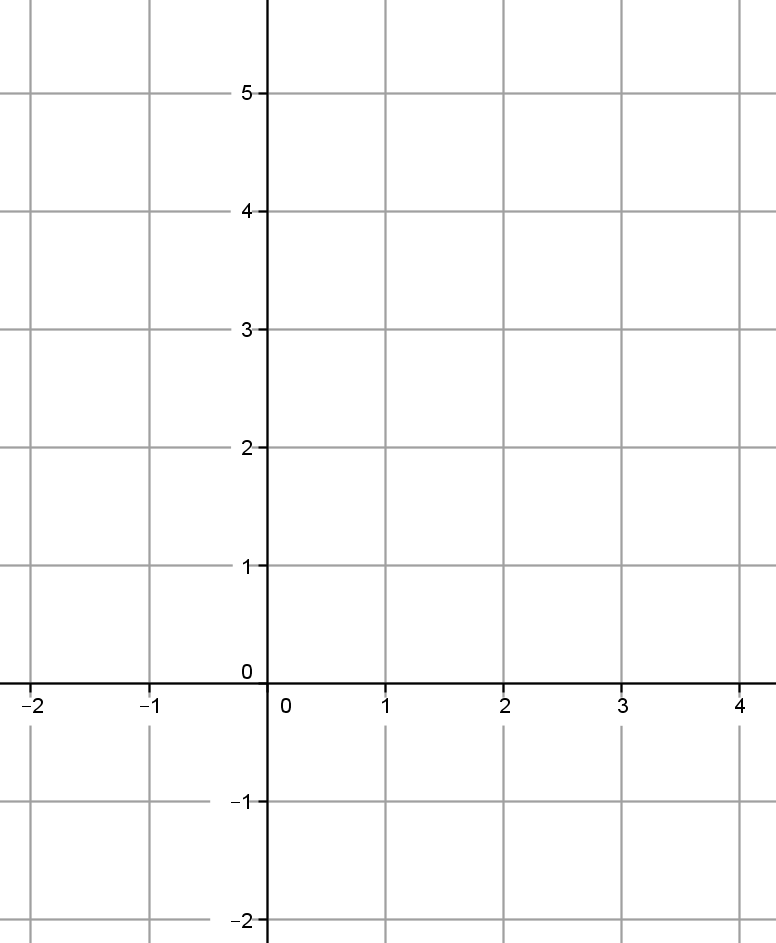
\includegraphics[width=55mm]{images/ex1.png}


\enskip

\textit{ex 44 p 159; ex 55 p 160; ex 51 p 160}

\section{D�terminer l'expression alg�brique d'une fonction affine}

\ul{Propri�t�:} On consid�re la fonction affine $f: x \mapsto ax+b$. Pour deux
nombres distincts $x_1$ et $x_2$, on a: 

$a=\dfrac{f(x_1)-f(x_2)}{x_1-x_2}$.

\bigskip

\ul{Remarque}: Cette propri�t� permet de d�terminer le coefficient $a$ d'une
fonction affine lorsque l'on connnait deux points de la courbe.

\bigskip

\ul{Exemple :} D�terminer l'expression alg�brique de la fonction affine $g$
repr�sent�e ci-dessous.

\enskip

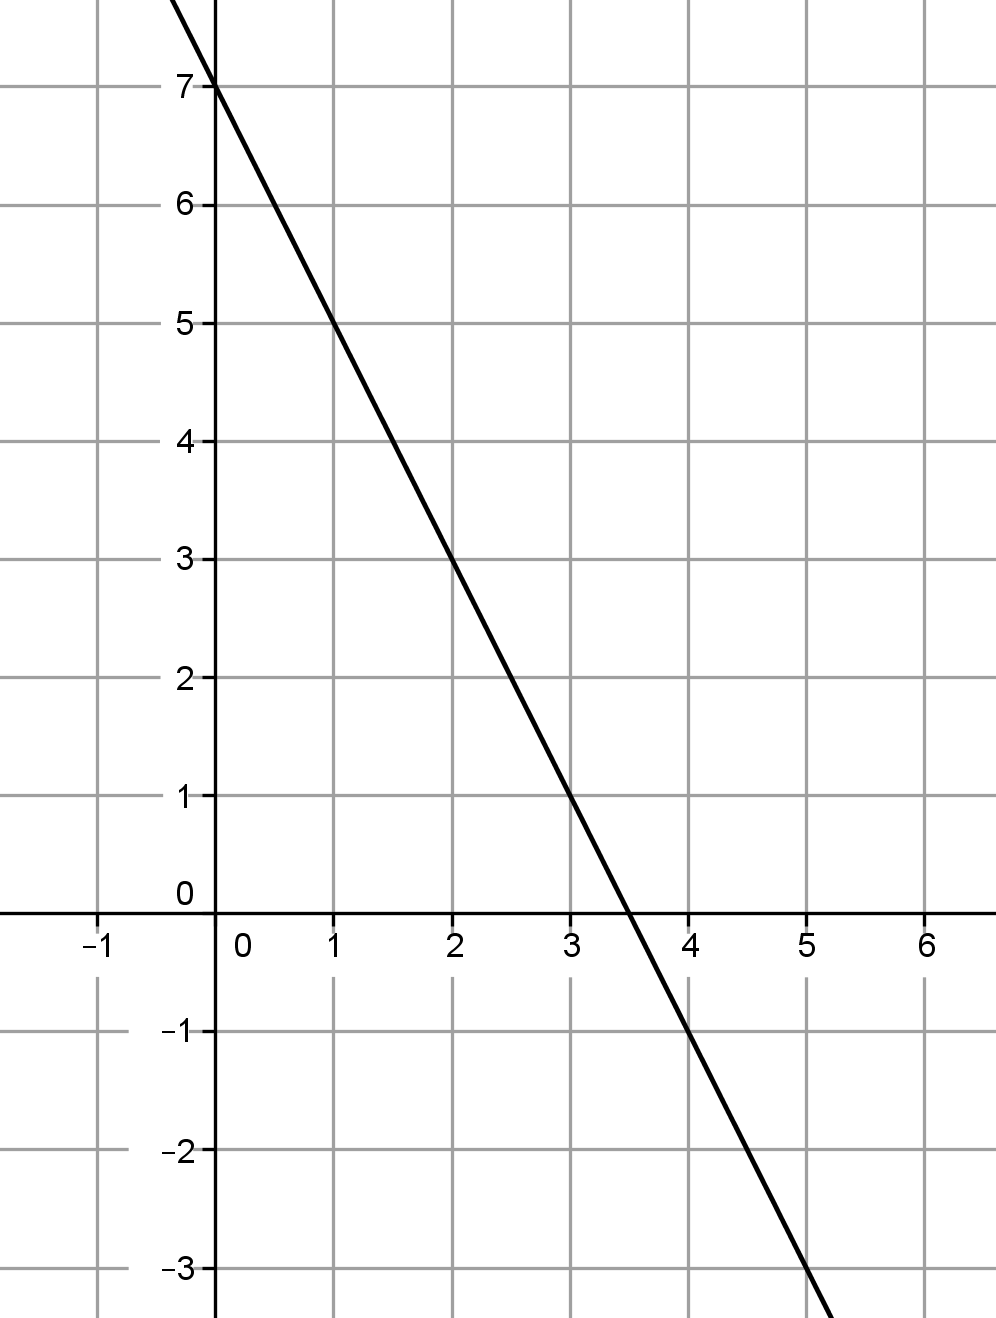
\includegraphics[width=8cm]{images/ex2.png}

\bigskip

\bigskip

\bigskip

\bigskip

\bigskip

\bigskip

\bigskip

\bigskip

\bigskip

\bigskip

\bigskip

\bigskip

\bigskip

\bigskip

\bigskip

\bigskip

\bigskip

\bigskip

\bigskip

\bigskip

\bigskip

\bigskip

\textit{ex 56 p 160; ex 57 p160; ex 59 p 161; ex 88 p 166.}
\end{document}
